\documentclass[hyperref={pdfpagelabels=true}]{beamer}

\usepackage{lmodern}
%%%%%%%%%%%%%%%%%%%%%%%%%%%%%%%%%%%%%%%%%%%%%%%%%%%%%%%%%%%%%%%%%%%%%%%%%%%%%%%%%%%%%%%%%%%%%%%%%
%This work is licensed under a Creative Commons Attribution-ShareAlike 4.0 International License.
%
%You are free to:
%
%    Share — copy and redistribute the material in any medium or format
%    Adapt — remix, transform, and build upon the material
%    for any purpose, even commercially.
%
%    The licensor cannot revoke these freedoms as long as you follow the license terms.
%
%Attribution — You must give appropriate credit, provide a link to the license, and indicate if changes were made. You may do so in any reasonable manner, but not in any way that suggests the licensor endorses you or your use.
%
%ShareAlike — If you remix, transform, or build upon the material, you must distribute your contributions under the same license as the original. 
%
%%%%%%%%%%%%%%%%%%%%%%%%%%%%%%%%%%%%%%%%%%%%%%%%%%%%%%%%%%%%%%%%%%%%%%%%%%%%%%%%%%%%%%%%%%%%%%%%%
\definecolor{dred}{rgb}{0.647059, 0.164706, 0.164706}
\definecolor{dgreen}{rgb}{0., 0.545098, 0.545098}
%\usecolortheme[named=dred]{structure}

\title{Big Data and Spatial Databases}
\subtitle{A Comparative Analysis}
\author{Joana Sim\~{o}es} 

\author[shortname]{Joana Sim\~{o}es \inst{1}, Rafael Gim\`{e}nez \inst{1}, Marc Planagum\`{a} \inst{1}}
\institute[shortinst]{\inst{1} Bdigital}

%\date{\today} 
%\titlegraphic{\includegraphics[width=.35\textwidth]{bigdata2.png}}
 
\usepackage{beamerthemeshadow}
%\usepackage{beamerthemesplit}
\usepackage{listings}

\newcommand{\soooo}{H$_2$SO$_4$}

%fdl stuff
\usepackage{hyperref}
\hypersetup{colorlinks, 
           citecolor=black,
           filecolor=black,
           linkcolor=black,
           urlcolor=black,
           bookmarksopen=true,
           pdftex}

\hfuzz = .6pt % avoid black boxes

\lstset{language=SQL}

\begin{document}
\setbeamertemplate{footline}[page number]
\setbeamertemplate{navigation symbols}{}
\begin{frame}
\titlepage

%\begin{titlepage}
%\centering{ 
%  \includegraphics[scale=0.2]{bigdata2.png}
%  \includegraphics[scale=0.2]{bigdata1.png}  
%}
%\end{titlepage}

\end{frame} 

 
\begin{frame}
\frametitle{Table of Contents}
%\tiny{
\tableofcontents%}
\end{frame}

\section{Introduction} 
\begin{frame}
\frametitle{Motivation}
    \begin{itemize}
     \item<1->The volume of geospatial data has increased largely in the past few years.
    \begin{itemize}
      \item<2->Cheaper and widely adopted positioning technologies.
      \item<3->Spatial crowd-sourcing movements/ Volunteer Geographic Information (VGI).%OSM, Ushahidi
      \end{itemize}
    \end{itemize}        
    \begin{figure}       
	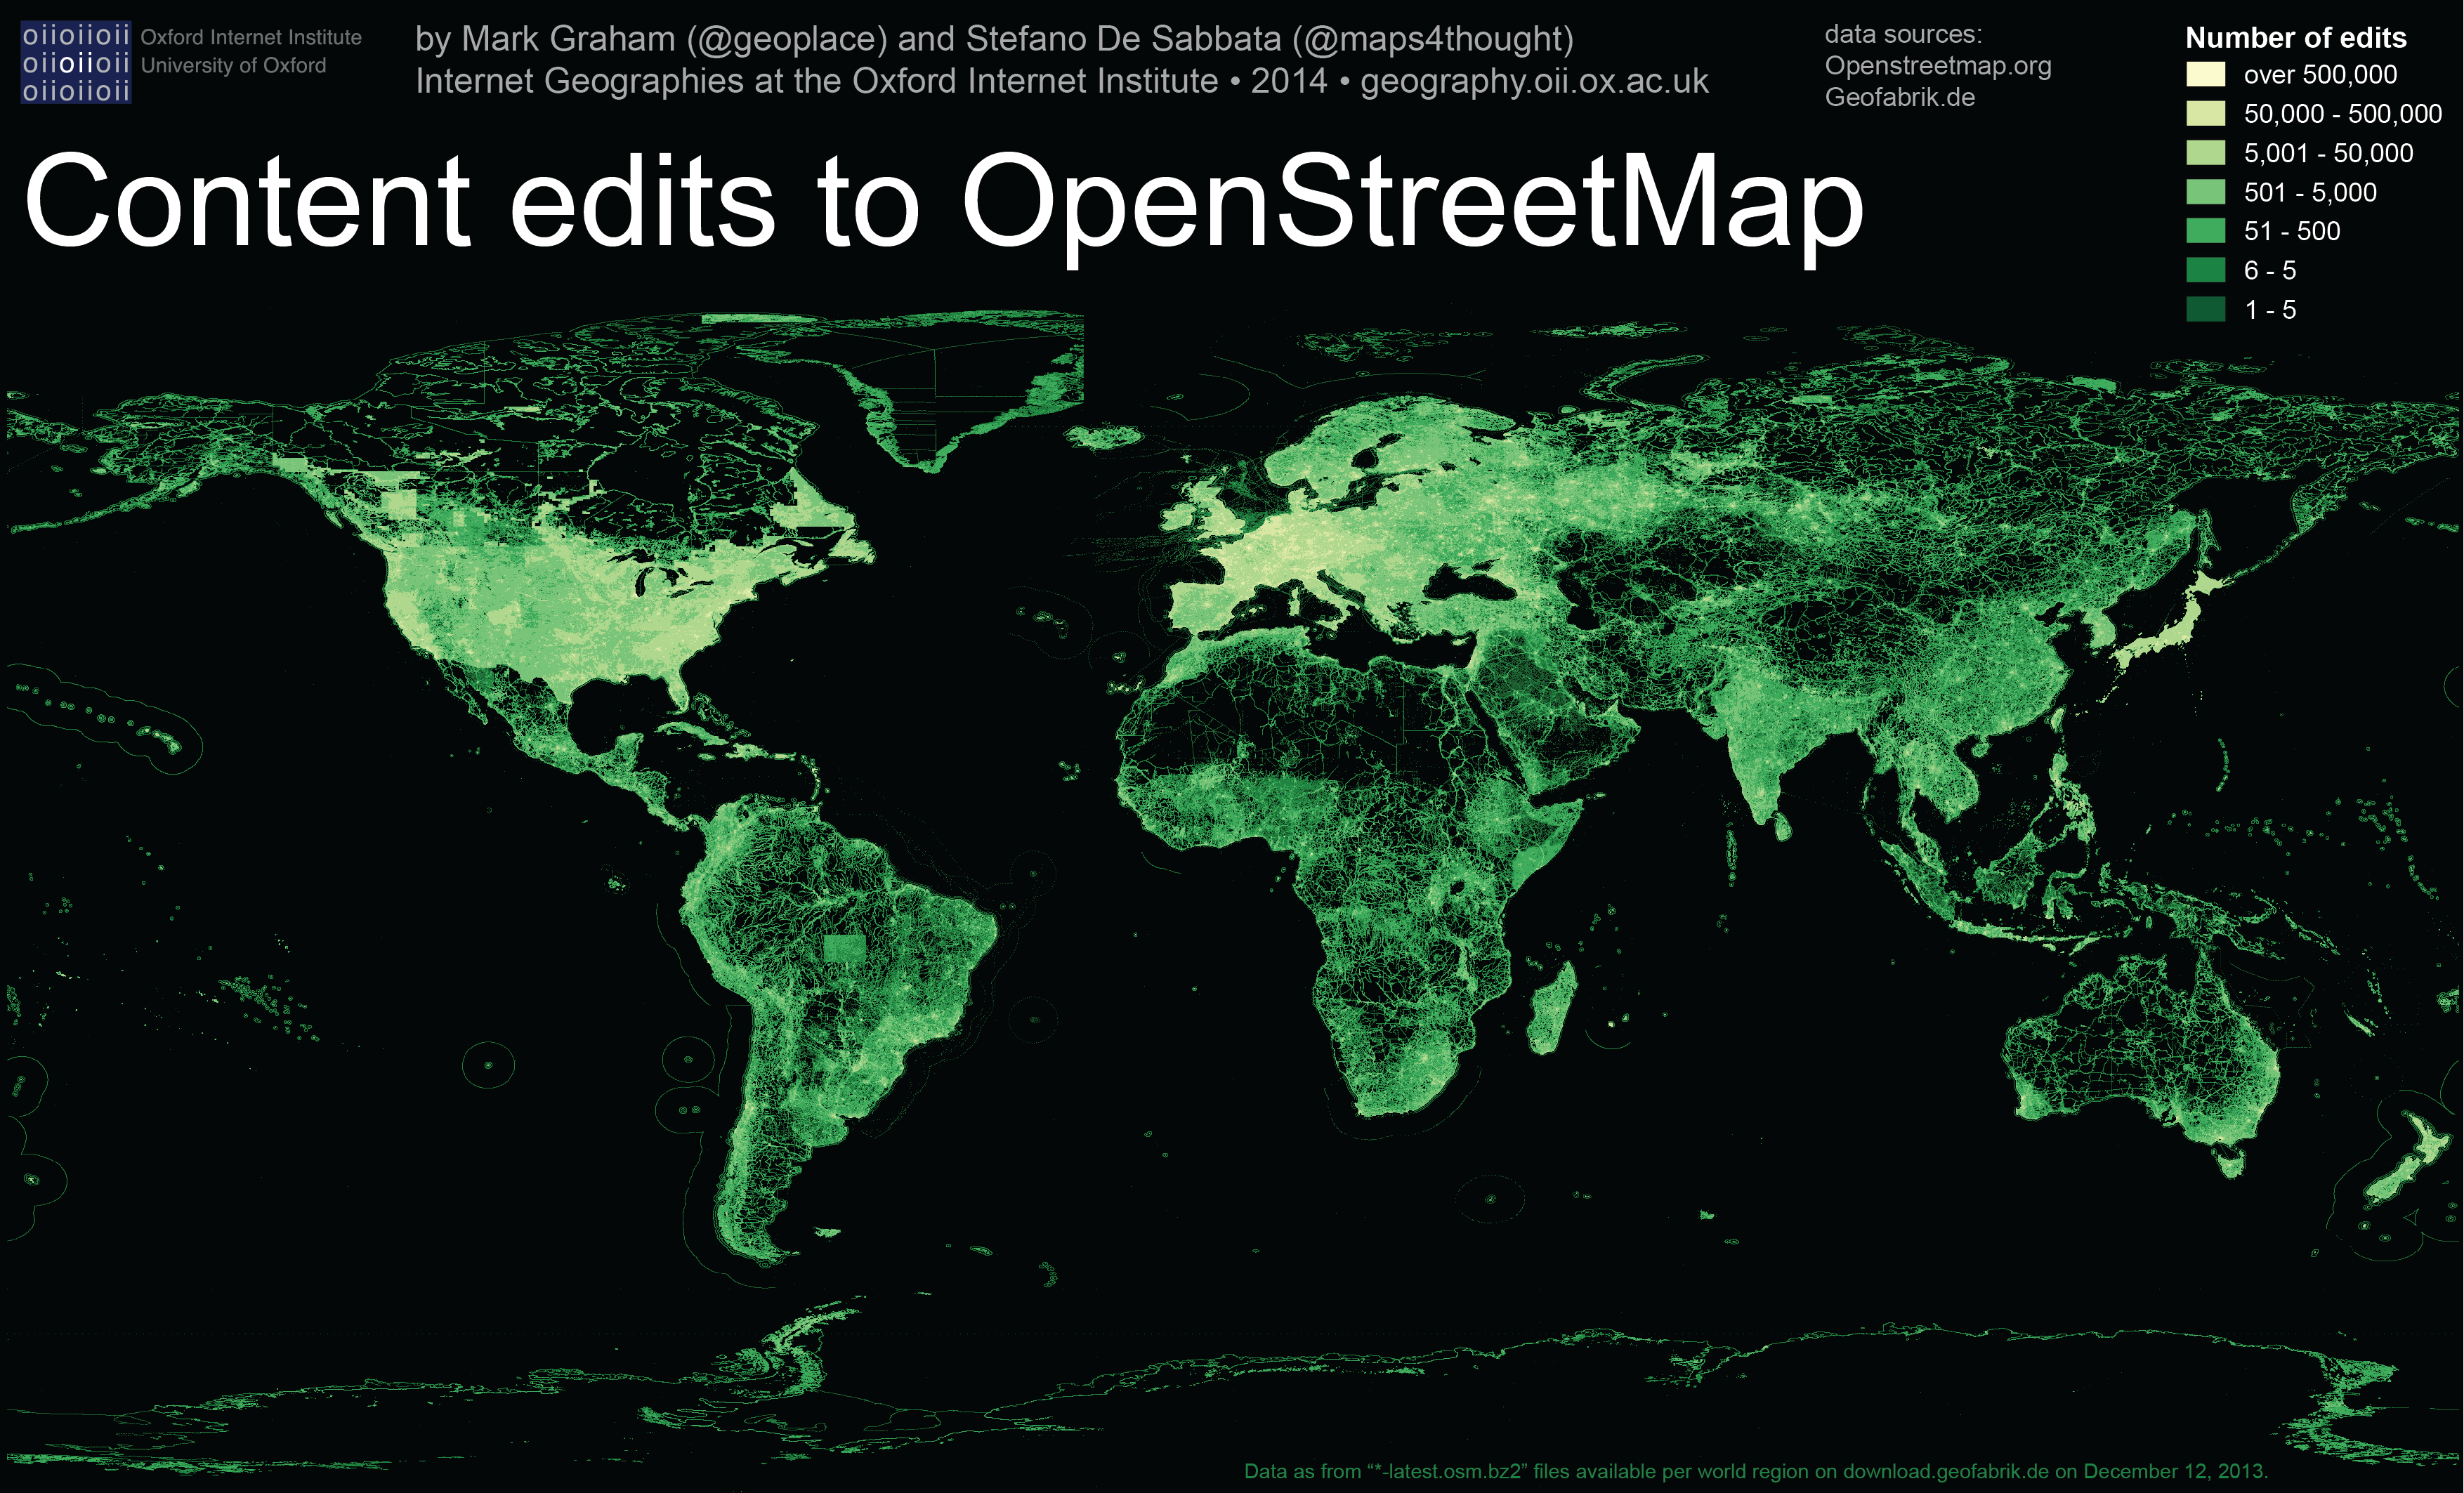
\includegraphics[width=0.6\textwidth]{osm.png}      
     \end{figure}      
\end{frame}

\begin{frame}
\frametitle{What is so \textit{Special} about \textit{Spatial}}
    \begin{itemize}
    \item<1->Spatial queries rely on geometrical operations, not only for \textbf{computing measurements} and \textbf{generating new objects}, but also as \textbf{logical operations for topology relationships}.% (e.g.: contains, intersects, touches). 
    \item<2->The increasing volume of spatial information, coupled with the computationally intensive nature of spatial queries demand scalable and efficient solutions.
    \begin{itemize}
      \item<3->fast query response, which requires a scalable architecture.
      \item<3->Support to clusters on a cost-effective architecture, such as commodity clusters or cloud environments.
     \end{itemize}
    \end{itemize}      
\end{frame}
 
\begin{frame}
\frametitle{Our Approach}
    \begin{itemize}
      \item<1->To track the performance of different spatial warehouse environments on the cloud, regarding a closed set of spatial queries.
      \item<2->To compare a relational database server running on a single-machine with different clusters.%more specifically
      \item<3->\textbf{Disclaimer:} we focused whithin the scope of our work environment.%queries that we use, samples that we use (that are not necessarily big), and infra structure/budget that we have.
    \end{itemize}
\end{frame}

\section{Benchmarking Setup} 
\begin{frame}
\frametitle{The cloud}
    \begin{figure}       
	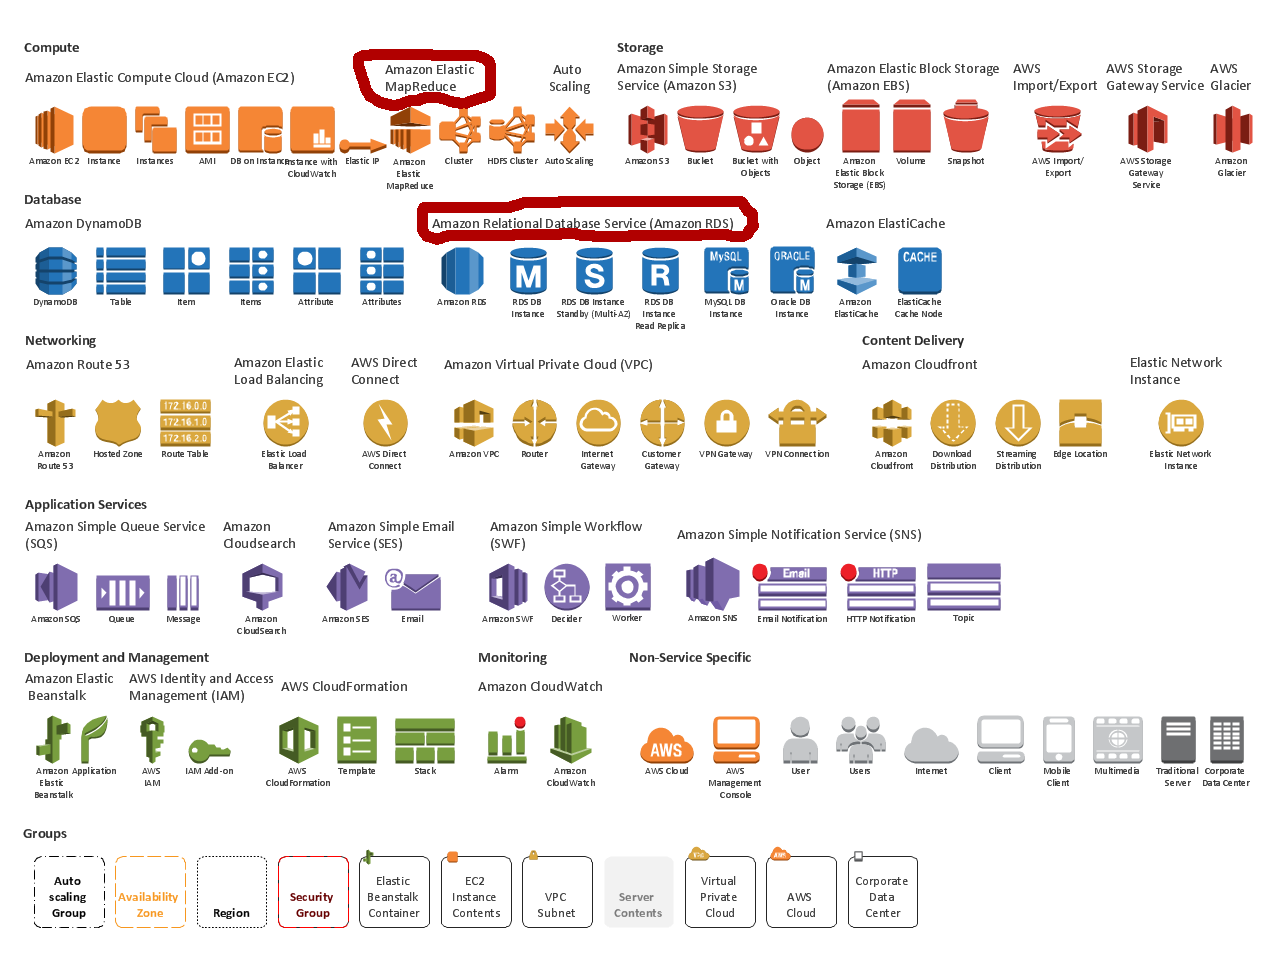
\includegraphics[width=0.8\textwidth]{cloud_aws1.png}      
     \end{figure}      
\end{frame}

\begin{frame}
\frametitle{RDS vs EMR}
\begin{columns}
  \begin{column}{0.5\textwidth}
   \textbf{Relational Database Service (RDS)}
   \begin{itemize}
    \item<2->RDBMS on a dedicated server, with an optimized configuration.
    \item<3->PostgreSQL v.9.3.3
    \item<3->PostGIS 2.1
    \end{itemize}
  \end{column}
  
  \begin{column}{0.5\textwidth}
  \textbf{Elastic Map Reduce (EMR)}
   \begin{itemize}
    \item<2->A Linux-based distributed system that uses Hadoop as framework.
    \item<3->Hadoop 2.4.0
    \item<3->Hive 0.13.1
    \item<3->\textbf{GIS tools for Hadoop 2.0}
    \end{itemize}  
  \end{column}  
\end{columns}
\end{frame}

\begin{frame}
\frametitle{Introducing GIS tools for Hadoop}
\begin{columns}
  \begin{column}{0.5\textwidth}
   \begin{itemize}  
    \item<2->FOS toolkit for "Big Spatial Data Analytics".%from ESRI. %github. Apache License
    \item<2->Hosted on github.
    \item<2->It consists in three libraries:
   \begin{itemize}    
      \item<2->Esri Geometry API for Java.
      \item<2->Geoprocessing Tools for Hadoop.
      \item<2->\textbf{Spatial Framework for Hadoop (SFH):} extends Hive to to enable spatial queries and geometry types.% It is based on the ESRI Geometry API for Java
    \end{itemize} 
   \end{itemize}     
 \end{column}  
  \begin{column}{0.5\textwidth}
    \begin{figure}       
	
\includegraphics[width=\textwidth]{gis4hadoop.png}      
     \end{figure}        
 \end{column}  
 \end{columns}  
\end{frame}

\begin{frame}
\frametitle{Hardware Description}
\begin{table}
\begin{tabular}{l | c }
Designation & Description \\
\hline \hline
RDS & db.m3.medium: 100 GB, 1 CPU, 3.75 GB RAM\\ 
EMRx3 & master: m3.xlarge; cores: m1.medium (3)\\
EMRx6 & master: m3.xlarge; cores: m1.medium (6)\\
EMRx9 & master: m3.xlarge; cores: m1.medium (9) \\
EMRx3Large & master: m3.xlarge; cores: m3.xlarge (3)\\
\end{tabular}
      \vspace{5mm}  
\begin{description}
\item[m1.medium] 410 GB, 3.75 GB RAM, 1 CPU:
\item[m3.xlarge] SSD 2x40 GB, 15 GB RAM, 4xCPU;  	
\end{description}

%\caption{Hardware Description}
\end{table}
\end{frame}

\section{The Queries} 
\begin{frame}
\frametitle{Introducing the Queries}
   \begin{itemize}    
      \item<1->Four queries.
      \item<1->Four Layers with different geometries (e.g: point, polygon, polyline).
      \item<1->Same CRS: Google Mercator (EPSG:3857).
      \item<1->Syntax may differ slightly on PostGIS and SFH.      
    \end{itemize} 
    \begin{figure}       
	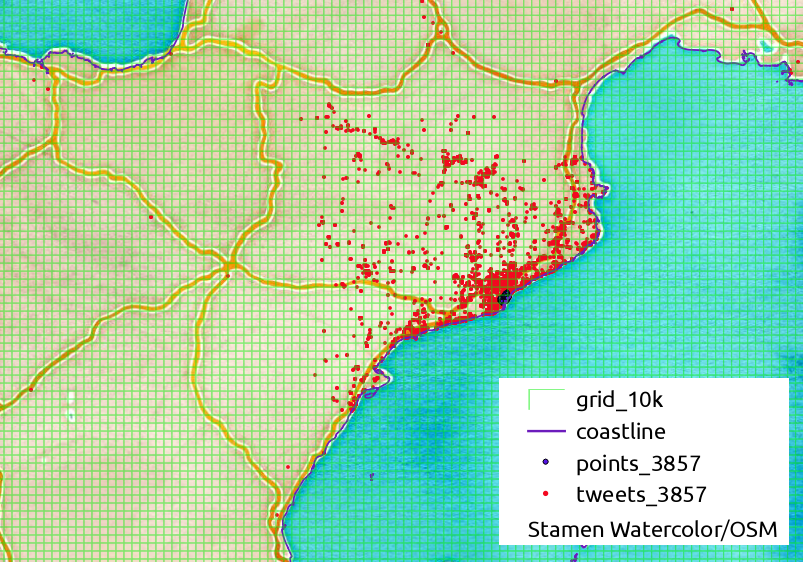
\includegraphics[width=0.5\textwidth]{layers_legend.png}      
     \end{figure}            
\end{frame}

\begin{frame}
\frametitle{Create Density Grid}
\begin{columns}
  \begin{column}{0.5\textwidth}
  \begin{itemize}    
    \item<1->Objective: transforming a point cloud in a density surface.
    \item<1->Scenario: create a grid for displaying the density of tweets.%10Km
    \item<1->Operations involved: create table, aggregation (GROUP BY), ST\_CONTAINS.    
  \end{itemize} 
 \end{column}  
  \begin{column}{0.5\textwidth}  
    \begin{figure}       
	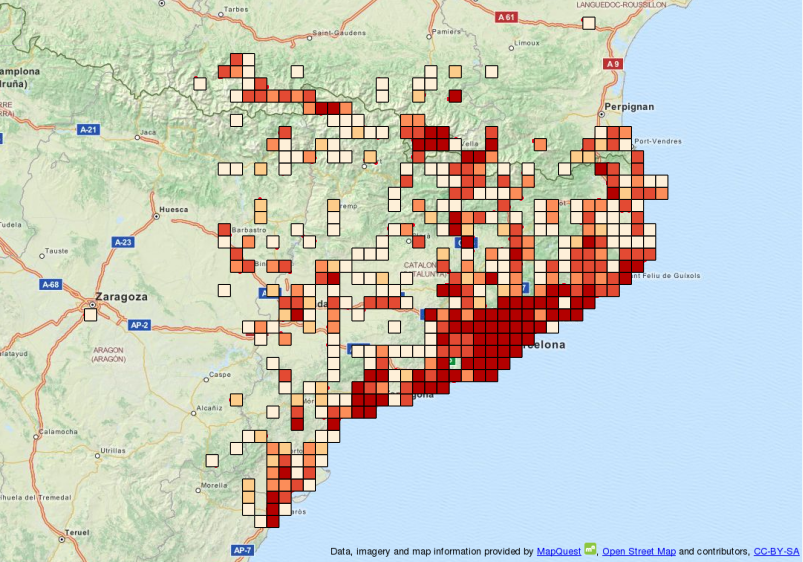
\includegraphics[width=\textwidth]{density.png}      
     \end{figure}            
 \end{column}  
\end{columns}      
\end{frame}

\begin{frame}
\frametitle{Buffers}
\begin{columns}
  \begin{column}{0.5\textwidth}
    \begin{itemize}    
      \item<1->Objective: count how many points lie whithin a buffer.
      \item<1->Scenario: how many tweets are sent within 100 m of a bicing station.%do people tweet a lot just before or after they use the bicing?
      \item<1->Operations involved: ST\_BUFFER, ST\_CONTAINS.    
    \end{itemize} 
 \end{column}  
  \begin{column}{0.5\textwidth}    
    \begin{figure}       
	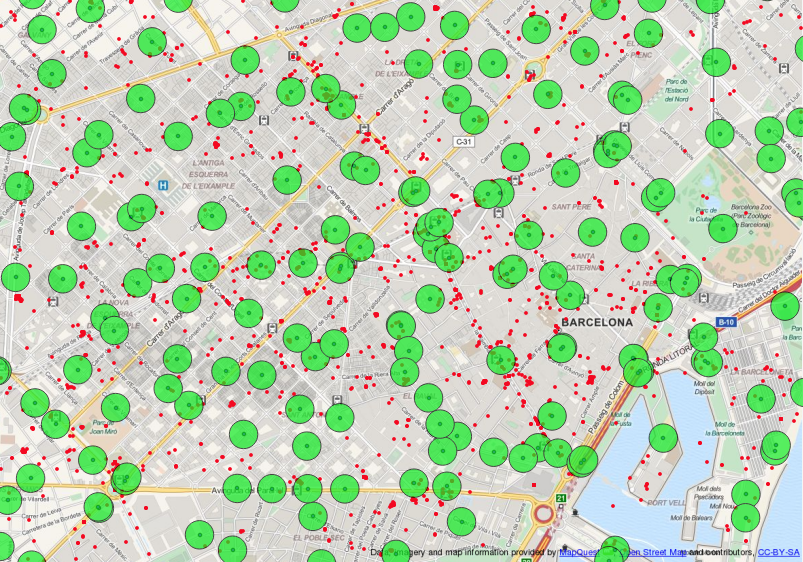
\includegraphics[width=\textwidth]{bicing.png}      
     \end{figure}            
 \end{column}  
\end{columns}           
\end{frame}

\begin{frame}
\frametitle{Select Maximum Distance}
\begin{columns}
  \begin{column}{0.5\textwidth}
  \begin{itemize}    
    \item<1->Objective: measure distance between two points.
    \item<1->Scenario: calculate the maximum distance between tweets mentioning New Years, on New Years Day (01/01/2015).
    \item<1->Operations involved: MAX, ST\_DISTANCE, filters (WHERE).    
  \end{itemize} 
 \end{column}  
  \begin{column}{0.5\textwidth}      
    \begin{figure}       
	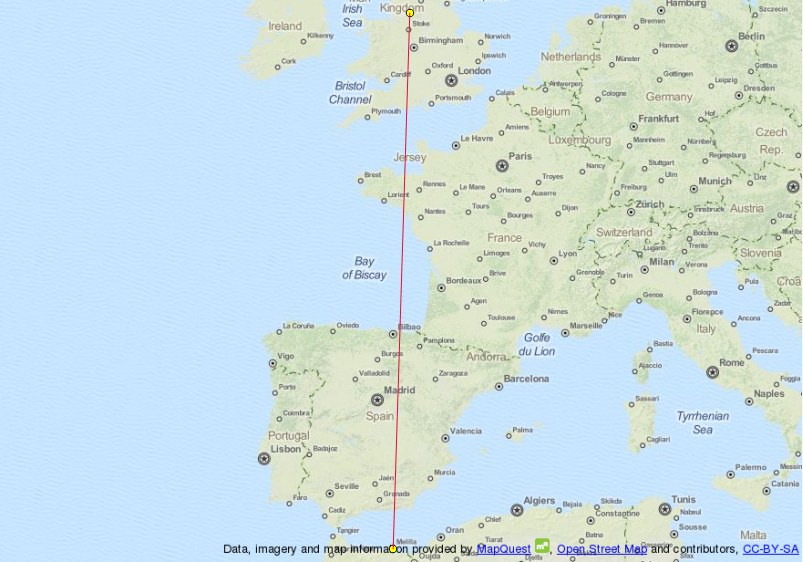
\includegraphics[width=\textwidth]{dist.png}      
     \end{figure} 
 \end{column}  
\end{columns}           
\end{frame}

\begin{frame}
\frametitle{Import Layer}
\begin{columns}
  \begin{column}{0.5\textwidth}
  \begin{itemize}    
    \item<1->Objective: importing a layer into the system.
    \item<1->Scenario: instantiate geometry from a CSV file, with WKT definitions.
    \item<1->Operations involved: create table, copy values, ST\_GeomFromText.    
  \end{itemize} 
 \end{column}  
  \begin{column}{0.5\textwidth}      
    \begin{figure}       
	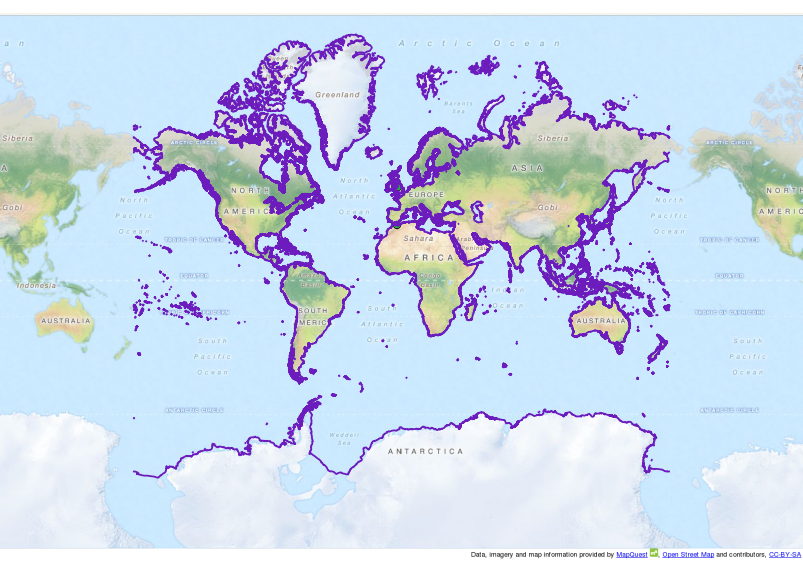
\includegraphics[width=\textwidth]{coastline.png}      
     \end{figure} 
 \end{column}  
\end{columns}           
\end{frame}

\begin{frame}
\frametitle{Running the Queries}
  \begin{itemize}    
    \item<1->Query times on clusters showed a large variability, so we used average values.% 10 runs.
  \end{itemize} 
\begin{figure}       
    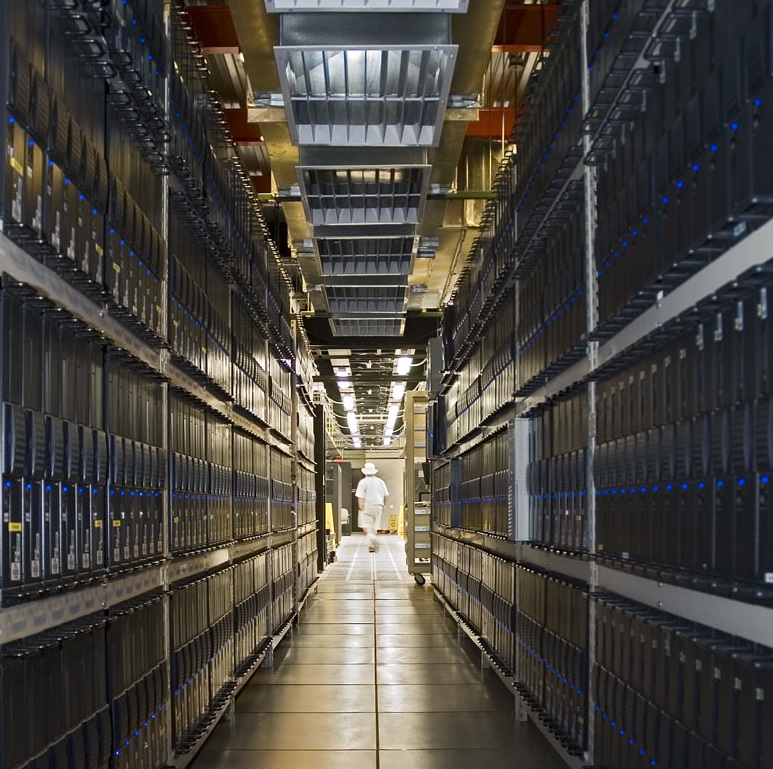
\includegraphics[width=0.5\textwidth]{modern_cluster.jpg}      
\end{figure}      
\end{frame}


\section{Results} 
\begin{frame}
\frametitle{General Overview}
  \begin{itemize}    
    \item<2->The \textit{buffers} query, is by far the most expensive one.
  \end{itemize} 
    \begin{figure}       
	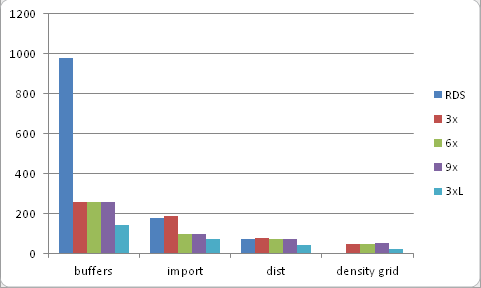
\includegraphics[width=0.6\textwidth]{general1.png}      
	\caption{\tiny{Results of the benchmarking of the different queries, on different setups on the cloud; query duration is shown in seconds.}}
     \end{figure} 
\end{frame}

\begin{frame}
\frametitle{Buffers}
  \begin{itemize}    
    \item<2->This is where RDS has its worst performance.
  \end{itemize} 
    \begin{figure}       
	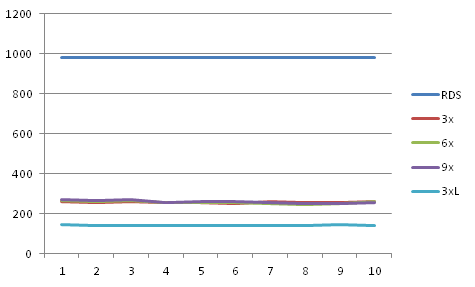
\includegraphics[width=0.6\textwidth]{buffers.png}      
	\caption{\tiny{duration of the \textit{buffers} query.}}
     \end{figure} 
\end{frame}

\begin{frame}
\frametitle{Import Layer}
  \begin{itemize}    
    \item<2->On this query RDS also performs much worst than any of the clusters.%the import process is quite different in both systems
    \item<3->Using an alternative method for importing (shp2pgsql) improves dramatically the import time for RDS.% 179 sec, better than the worst cluster    
  \end{itemize} 
    \begin{figure}       
	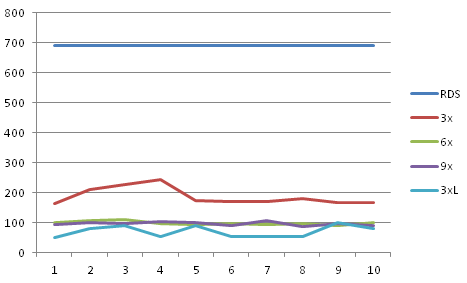
\includegraphics[width=0.6\textwidth]{import.png}      
	\caption{\tiny{duration of the \textit{import} query.}}
     \end{figure} 
\end{frame}

\begin{frame}
\frametitle{Create Density Grid}
  \begin{itemize}    
    \item<2->RDS is 20 to 50 times faster than the clusters.%best performance
    \item<3->Using more workers (9), actually results in longer response times.
  \end{itemize} 
    \begin{figure}       
	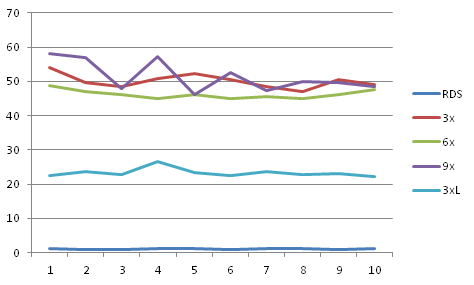
\includegraphics[width=0.6\textwidth]{grid.png}      
	\caption{\tiny{duration of the \textit{grid} query.}}
     \end{figure} 
\end{frame}

\begin{frame}
\frametitle{Select Maximum Distance}
  \begin{itemize}    
    \item<2->Second less expensive query.
    \item<3->RDS performs better than the smaller cluster (EMRx3).
  \end{itemize} 
    \begin{figure}       
	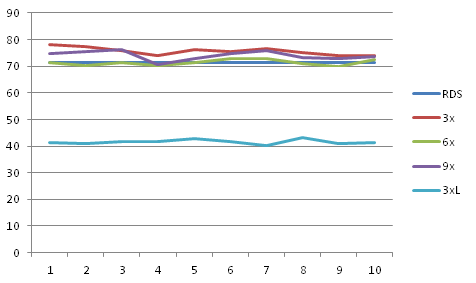
\includegraphics[width=0.6\textwidth]{dist2.png}      
	\caption{\tiny{duration of the \textit{distance} query.}}
     \end{figure} 
\end{frame}

\begin{frame}
\frametitle{\$\$\$}
  %\begin{itemize}    
   % \item<1->The costs bellow were calculated using the AWS calculator.
    %\item<1->Since all the queries were completed in less than 1 hour, we used the cost of 1h/mnth.
  %\end{itemize} 
    \begin{figure}       
	
\includegraphics[width=0.7\textwidth]{money.png}      
     \end{figure} 
\end{frame}

\begin{frame}
\frametitle{Costs}
  \begin{itemize}    
    \item<1->The costs bellow were calculated using the AWS calculator.
    \item<1->Since all the queries were completed in less than 1 hour, we used the cost of 1h/mnth.
  \end{itemize} 
    \begin{figure}       
	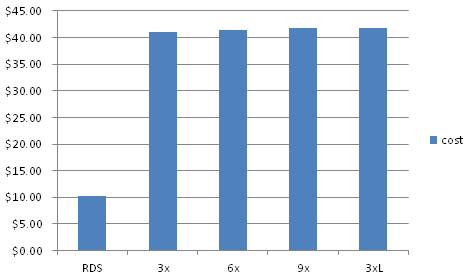
\includegraphics[width=0.6\textwidth]{cost.png}      
	\caption{\tiny{Cost in dollars, for deploying each benchmarking environment in AWS.}}
     \end{figure} 
\end{frame}

\begin{frame}
\frametitle{Time for Some Conclusions?}
  \begin{figure}       
      
\includegraphics[width=0.5\textwidth]{think.jpg}      
    \end{figure} 
\end{frame}

\section{Conclusions} 
\begin{frame}
\frametitle{Disruptive Conclusions}
  \begin{itemize}    
    \item<2->Don't throw PostgreSQL away: a cluster is not \textbf{always} preferable to RDS.%smaller queries don't gain anything to run in a cluster; confirmed by better performance in less expensive queires
    \item<3->Adding nodes to a cluster does \textbf{not} necessarily result in a better performance.%explanations: extra burden of having to distribute the workload is not compensated in gains in terms of performance; how much ESRI is actually taking advantage of the MT paradigm?
    \item<4->It was nearly always the case, that the best performance was achieved using a small cluster with \textit{large} machines.%vertical scalability instead of horizontal scalability
    \item<5->Price-wise, RDS and EMRx3Large are good deals.% The smaller price difference justifies the boost in performance
    \item<6->On the context of this benchmarking, the cluster with more nodes (EMRx9) seems like a waste of money.
    \item<7->These disruptive results enforce the urge to do more benchmarkings, with larger sample sizes, and to review the code from SFH.%or find something else    
  \end{itemize} 
\end{frame}

\begin{frame}
\frametitle{References}
\begin{itemize}
\tiny{
\item Dunning, T. and Friedman, E. (2014) Time Series Databases: New Ways to Store and Access Data. O'Reilly Media; 1 edition.
\item OpenStreetMap. OpenStreetMap. Retrieved March 9, 2015, from: \url{https://www.openstreetmap.org/}
\item Ushahidi. Ushahidi. Retrieved March 9, 2015, from: \url{http://www.ushahidi.com/}
\item Aji, A.; Wang, F.; Vo, H.; Lee, R.; Liu, Q.; Zhang, X. \& Saltz, J. (2013). Hadoop-GIS: A High Performance Spatial Data Warehousing System over MapReduce. Proceedings of the VLDB Endowment International Conference on Very Large Data Bases, 6(11), p1009.
\item Amazon. Amazon Web Services. Retrieved March 15, 2015, from: \url{https://aws.amazon.com/}
\item PostgreSQL. PostgreSQL. Retrieved March 15, 2015, from: \url{http://www.postgresql.org/}
\item License. PostgreSQL. Retrieved March 9, 2015, from: \url{http://www.postgresql.org/about/licence/}
\item PostGIS. Spatial and Geographic objects for PostgreSQL. Retrieved March 9, 2015, from: \url{http://postgis.net/}
\item Apache. Hadoop. Retrieved March 9, 2015, from: \url{https://hadoop.apache.org/}
\item The Apache Software Foundation. Apache License, Version 2.0. Retrieved March 15, 2015, from: \url{http://www.apache.org/licenses/LICENSE-2.0}
\item ESRI. Spatial Framework for Hadoop. Retrieved March 15, 2015, from: \url{https://github.com/Esri/spatial-framework-for-hadoop}
\item ESRI.  Spatial Framework for Hadoop license. Retrieved March 15, 2015, from: \url{https://github.com/Esri/spatial-framework-for-hadoop/blob/master/license.txt}
\item Stolze, K. SQL/MM Spatial: The Standard to Manage Spatial Data in Relational Database Systems. Retrieved March 15, 2015, from: \url{http://doesen0.informatik.uni-leipzig.de/proceedings/paper/68.pdf}
\item Wikipedia. Bicing. Retrieved March 15, 2015, from: \url{https://en.wikipedia.org/wiki/Bicing}
\item Stack Overflow. What is the best hack for importing large datasets into PostGIS? Retrieved March 9, 2015, from: \url{http://gis.stackexchange.com/questions/109564/what-is-the-best-hack-for-importing-large-datasets-into-postgis}
\item Amazon Web Services. Simple Monthly Calculator. Retrieved March 9, 2015, from \url{https://calculator.s3.amazonaws.com/index.html}
}
\end{itemize}
\end{frame}

\begin{frame}
\frametitle{Thank You!}
    \begin{figure}   
      
\includegraphics[width=0.2\textwidth]{thanks.jpg}      
    \end{figure}   
    This presentation is available at: \centering{\\ \url{http://tinyurl.com/q9rh3co}\\}
      \vspace{5mm}    
\end{frame}


\end{document}